\documentclass{article}

\usepackage[spanish=nohyphenation]{hyphsubst}
\usepackage[spanish]{babel}
\usepackage[utf8]{inputenc}
\usepackage{fullpage}
\usepackage{minted}
\usepackage{xspace}
\usepackage{graphicx}
\usepackage{enumitem}
\usepackage{multicol}
\usepackage[colorlinks=true, linkcolor=blue]{hyperref}

\newcommand{\fgp}{\textbf{FreeGeomPhy}\xspace}
\newcommand{\fgpv}{v. 0.5\xspace}
\newcommand{\cfgp}{\fgp \fgpv}

\newcommand{\refpar}[1]{\S\ref{#1}}
\newcommand{\refsec}[1]{(véase \refpar{#1})}

\title{Documentación del paquete \cfgp para Octave}

\author{Aarón Bueno Villares \textless abv150ci@gmail.com\textgreater \thanks{Tutorizado por
    Cated\textsuperscript{co}. Pedro L. Galindo Riaño}}
\date{\today}

\begin{document}
\maketitle
\setcounter{tocdepth}{2}
\tableofcontents

\section{Introducción}
\label{sec:intro}
El paquete \fgp es un paquete Octave con una colección de objetos para
representación de funciones, (in)ecuaciones, sistemas de (in)ecuaciones,
figuras geométricas y entidades físicas. Su utilidad es la de
poder definir la geometría de un objeto físico y obtener el valor de
las propiedades físicas deseadas en puntos de él.

En la versión actual de \fgp, \fgpv, no se ha desarrollado el manejo
de las propiedades físicas de un objeto dado, por lo que sólo se
dispone de figuras geométricas y las operaciones asociadas con él.

\subsection{Definiciones}
\begin{description}
  \item[Figura] Sinónimo de figura geométrica, definida como un
    conjunto de puntos que satisfacen una serie de propiedades
    modeladas mediante un sistema de ecuaciones e inecuaciones.
  \item[Entidad física] Figura con una serie de carácterísticas o
    propiedades físicas, modeladas mediante una colección de
    funciones, una por característica física.
\end{description}

\section{Estructura de directorios de \fgp}
\label{sec:struct}
El paquete \fgp dispone actualmente de 5 clases llamadas
\texttt{hfunction}, \texttt{hequation}, \texttt{hsystem},
\texttt{hfigure} y \texttt{hcube}, cada una de las cuales están
implementadas en las carpetas \texttt{@hfunction},
\texttt{@equation}, \texttt{@hsystem}, \texttt{@hfigure} y
\texttt{@hcube}, tal y como exige exige Octave para la definición de
clases.

Dentro de cada una de dichas carpetas tenemos implementadas el
constructor y cada uno de los operadores y funciones definidas para la
clase en cuestión.

Además, disponemos del \textit{script} \texttt{loadPack}, que carga a
las variables \texttt{hX, hx, hy, hz} y \texttt{hend}, y las funciones
\texttt{hh}, \texttt{hn}, \texttt{hv}, \texttt{hc}, \texttt{he} y
\texttt{hpi}.

Por último, dispone de la carpeta \texttt{doc} que contiene el código
de ésta documentación.

Como podemos observar, todas las clases, variables y funciones extra
contienen el prefijo \textbf{h}. El motivo es que la primera clase que
se implementó, la correspondiente al manejo de funciones, y para
evitar ambigüedad con la función \texttt{function} de Octave, se llamó
\texttt{hfunction}, donde dicha \textbf{h} se puede leer o interpretar
como \textit{handle} (manejador), ya que una \texttt{hfunction} no es
más que un manejador de una función. De hecho, las funciones se
construyen haciendo uso de la función \texttt{inline} de Octave que
permite crear manejadores a función escribiendo dicha función en una
cadena de carácteres. Así, todas las clases, operadores y funciones se
pueden leer o interpretar como \textbf{manejador a}.

\section{Clase \texttt{hfunction}}
\label{sec:hfun}
Esta clase, aun no siendo la más compleja, sí que es la que dispone de
un mayor número de detalles, y por tanto, es la clase más compleja y
larga de documentar, así que esta sección será bastante más larga que
las restantes secciones. Permite definir y transformar funciones
matemáticas con una serie de operadores diseñados para tal fin. El
nombre \texttt{hfunction} significa \textit{function handle},
colocando la h de \textit{handle} como prefijo, convenio que se
seguirá usando para el resto de clases del paquete.

Esta clase se usa principalmente para dar un trato unificado al manejo
de funciones por parte de clases más grandes como la de sistemas de
ecuaciones o figuras como cubos y esferas. En la mayoría de los casos,
quizás sea el usuario el que quiera definir su propia función para
definir, por ejemplo, una de las caras de un cubo. En este punto, la clase
\texttt{hfunction} permite crear una capa de abstracción entre los
detalles internos y el paso de parámetros de las funciones definidas
por el usuario, de modo que las figuras tratan a todas estas funciones
y su paso de parámetros de forma unificada.

Como veremos en \refpar{ssec:samples} trabajar con funciones
relativamente complejas usando la clase \texttt{hfunction} no es
quizás la solución más adecuada, sobre todo por cuestiones de claridad
y facilidad de uso. Para programar funciones complejas, quizás es
mejor que se programe la función en un fichero propio. El uso o
utilidad propia de esta clase desde el punto de vista del usuario
final\footnote{Como se ha comentado anteriormente, la clase tiene un
  propósito específico para las restantes clases del paquete} es
precisamente permitir realizar modificaciones \textit{inline},
mediante composición, a la función principal, con el fin de poder
realizar pruebas con bastante sencillez y visualizar los resultados;
ya no solo desde el punto de vista de una función en sí, sino desde el
punto de vista de las figuras geométricas que usan funciones para su
propia definición. Facilita mucho realizar modificaciones a las
funciones que se usan para definir figuras geométricas, y ver el
resultado de la propia figura.

Para saber cómo se usa dicha clase, empecemos por un ejemplo de uso
sencillo:

\begin{minipage}{0.4\textwidth}
\begin{minted}[linenos, frame=lines]{octave}
loadPack;

hf = hx .^ 2 + hy .^ 2;

plot3(hf, -1, 0.02, 1);
\end{minted}
\end{minipage}
\begin{minipage}{0.6\textwidth}
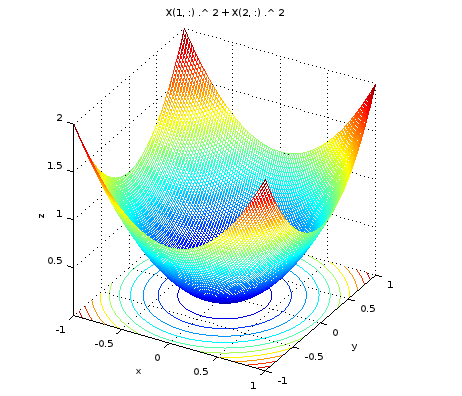
\includegraphics[scale=0.6]{figure1.png}
\end{minipage}

La primera línea de código solamente carga las variables \texttt{hx} y
\texttt{hy} que usamos a continuación. En realidad carga algunas
variables más, que veremos más adelante~\refsec{ssec:draw}.

Las variables \texttt{hx} y \texttt{hy} son dos
\texttt{hfunction} que representan a las funciones $f(X) = X(1, :)$ y
$f(X) = X(2, :)$. En consecuencia, \texttt{hf} representa a la función
$f(X) = X(1, :) ^ 2 + X(2, :) ^ 2$, que es precisamente la función que
estamos dibujando con la última línea. En ésta, le indicamos como
primer parámetro la función a dibujar, y los tres parámetros restantes
representan el intervalo sobre el que se calculará la función, tanto
en la coordenada $x$ como en la $y$. Es decir, en este caso, estamos
dibujando la función en el intervalo $(-1, 1)$ en $x$ y en el
intervalo $(-1, 1)$ en $y$ con incrementos de $0.02$, equivale al
vector \texttt{-1:0.02:1}~\refsec{sssec:spfuns}.

Las otras variables cargadas por \texttt{loadPack} son \texttt{hX},
que representa sin más a la función $f(X) = X$, \texttt{hz}, para
$f(X) = X(3, :)$ y \texttt{hend}, cuyo uso veremos más
adelante~\refsec{ssec:ref}.

\subsection{Matriz de puntos}
\label{ssec:matrix}
La clase \texttt{hfunction} supone que los datos vienen presentes en
una matriz de dimensión $2\times n, n\leq 1$ representando a una
matriz de $n$ puntos bidimensionales, es decir, los distintos puntos
son las diferentes columnas $X(:, i)$ de la matriz, siendo el conjunto
de coordenadas $x$ la primera fila, y el de $y$ la segunda. A su
vez, una función, al evaluarse sobre una matriz de estas
características, devuelve un vector fila con la coordenada $z$
correspondiente a cada punto.

\subsection{Otros parámetros adicionales}
\label{ssec:params}
A las funciones se les pueden pasar otros parámetros o argumentos que quizás
sean necesarios para realizar el cálculo: por ejemplo, definiendo una
función paramétrica (familias de funciones) que necesita de un
parámetro extra para quedar completamente especificado. Esto se detallará
en el apartado que viene a continuación.

\subsection{Las diferentes \texttt{hfunction}}
\label{ssec:constr}
Aunque la clase \texttt{hfunction} dispone de un constructor, no debe
ser llamado directamente y, para ello, el paquete dispone de una serie
de funciones auxiliares que devuelven objetos \texttt{hfunction}
construidos correctamente:

\begin{description}[font = \normalfont\itshape]
\item[hc(n)] Función constante $f(X) = n$, siendo $n$ un número
  cualquiera.
\item[hv(v)] Función identidad $f(X, v) = v$, siendo $v$ un nombre de
  variable válido.
\item[hh(h, $v_1$, $\ldots$, $v_n$)] Crea la función $f(X, v_1, \ldots,
  v_n) = h(v_1, \cdots, v_n)$. El parámetro $h$ debe ser un
  manejador de función válido de octave, y los parámetros $v_1,
  \ldots, v_n$ nombres de variables válidos. El nombre de la función
  puede leerse como manejador a manejador o \texttt{handle-handle}.
\item[he] Devuelve la función constante $f(X) = e$, siendo $e$ el
  número de Euler.
\item[hpi] Devuelve la función constante $f(X) = \pi$.
\end{description}

Es importante advertir que en todos estos casos, tenemos a $X$ como
primer parámetro. Esta es una asumpción necesaria ya que es el
parámetro de referencia, tanto para poder dibujar la función como para
trabajar con comodidad con sistemas de ecuaciones y figuras. A su vez,
es importante tener en cuenta que estas funciones son tomadas siempre
como funciones matemáticas y no como funciones de Octave a modo de
procedimiento. Este punto es importante para saber qué tipo de
modificadores y operadores podrán ser usados con él.

Veamos ahora como usar estas funciones:

\begin{minted}[linenos, frame=lines]{octave}
const_fun = hc(3)
var_fun = hv("k")
fun_fun = hh(@mod, "a", "b")
other_fun = const_fun + var_fun + fun_fun * he * hpi
\end{minted}

Que, al ejecutarlo, nos muestra en la salida del intérprete:

\begin{minted}[linenos, frame=lines]{octave}
f(X) = 3
f(X, k) = k
f(X, a, b) = mod(a, b)
f(X, k, a, b) = 3 + k + mod(a, b) * e * pi
\end{minted}

En realidad, podemos trabajar con variables y constantes de una forma
mucho más sencilla, por ejemplo, todas estas intrucciones son válidas:

\begin{minted}[linenos, frame=lines]{octave}
const_fun + 3 + fun_fun
fun_fun ^ "h"
var_fun + "z" + 3 * "b"
\end{minted}

Que produce las siguientes salidas:

\begin{minted}[linenos, frame=lines]{octave}
f(X, a, b) = 3 + 3 + mod(a, b)
f(X, a, b, h) = mod(a, b) ^ h
f(X, k, z, b) = k + z + 3 * b
\end{minted}

Esto nos podría llegar a concluir que las funciones \texttt{hn}
(función constante) y \texttt{hv} (función identidad) no sirven para
nada ya que no necesitamos llamarlas directamente como acabamos de
ver. Pero hay que tener cierto cuidado, ya
que la clase \texttt{hfunction} transforma todos los resultados
intermedios a objetos de la clase, y luego los combina usando los
operadores, pero si en la expresión no hay ningún objeto
\texttt{hfunction}, los operadores son tratados directamente por
Octave. Efectivamente, en este caso la expresión no sería de tipo
\texttt{hfunction} y la clase no puede hacer nada por evitarlo, puesto
que no está presente en la expresión (no podemos pretender que 3 + 4
no sea 7 y sí $f(X) = 3 + 4$).

Aún es más, debido a que los operadores tienen, en su gran mayoría de
casos, asociatividad izquierda, una expresión como \texttt{3 + "k"{} +
  fun\_fun} se resolvería como \texttt{((3 + "k"{}) + fun\_fun)}, y luego
al resultado indeseable \texttt{110 + fun\_fun}, ya que Octave
promociona \texttt{"k"} a entero, cuyo valor ASCII es 107, y le suma 3,
produciendo la función no pretendida \texttt{f(X, a, b) = 110 + sum(a,
  b)}. Para estos casos extraños es cuando puede ser útil las
funciones \texttt{hn} y \texttt{hv}.

De igual forma, puedo ejecutar una expresión como \texttt{fun\_fun +
  @sum} que también es aceptado sin discusión, pero, debido a que no
hay forma aquí de especificar los parámetros de la función
\texttt{sum}, se construiría el objeto \texttt{f(X, a, b) = mod(a, b)
  + sum()}.

\subsection{Cálculo de las funciones}
\label{ssec:calc}
Una vez que tenemos un objeto \texttt{hfunction}, para calcular sus
valores se procede como con una función normal:

\begin{minted}[linenos, frame=lines]{octave}
loadPack;

myFun = hx .^ 2 + hy .^ 2;

myFun([1 2; 3 4])
\end{minted}

Que produce como salida al vector $(1^2 + 3^2, 2^2 + 4^2) = (10,
20)$. En el caso de que al primer parámetro $X$ no lo necesitemos,
como en el inútil caso anterior $other\_fun \equiv f(X, h, a, b) = 3 +
h + mod(a, b)$, podemos ejecutar sin vergüenza $f([], 3, 8, 5)$, que
devolvería 9, aunque en este caso significa que alguna de las
variables $h$, $a$ o $b$ debería ser llamada $X$, los argumentos
adicionales deben ser usados (o se debe pensar en ellos) como
parámetros de la función a computar y no como los propios puntos del
dominio de definición de la misma.

\subsection{Órden de los argumentos}
\label{ssec:order}
Si solamente trabajamos con las hfunciones (así lo denominaré de ahora
en adelante) \texttt{hx}, \texttt{hy}, \texttt{hn} o constantes, y
cualquier otra que no implique la introducción de nuevas variables a
la hfuncion en construcción, toda hfunción tendrá un único parámetro
$X$, y a la hora de calcular los valores de la función éste será el
único argumento a considerar. Si al "<llamar"> a la hfunción, y pongo
"<llamar"> entrecomillado debido a que una hfunción no es un
procedimiento ---o no está diseñado para pensar en él de esa forma, como
ya hemos indicado---, con más parámetros de los específicados, éstos
serán ignorados, del mismo modo que pasa con las llamadas a funciones
normales de Octave.

En caso de que una hfunción tenga parámetros adicionales además de
$X$, el órden de estos parámetros vendrá determinado por el órden en
que aparezcan en la descripción de la misma, con la excepción del
parámetro $X$, que siempre va el primero. Por ejemplo: \texttt{hx +
  'h' + hh(@sum, a, b)} tendrá como parámetros $X, h, a, b$ y en ese
órden. Los parámetros de una hfunción se pueden consultar visualizando
la definición de la función (sin poner punto y coma al final) o
gracias a la función \texttt{argnames(h)}, que recibe una hfunción
\texttt{h} y devuelve la celda de cadenas de sus parámetros, que
coinciden en órden con el de evaluación.

Si a una hfunción le vamos añadiendo mediante el uso de operadores
(suma, división, etcétera) nuevas hfunciónes, los parámetros se irán
combinando mantiendo su órden relativo de aparición. Por ejemplo, si
sumamos dos hfunciones, basta visualizar cada una de ellas y luego la
hfunción recién construida para comprobar esta afirmación.

En caso de que al combinar dos hfunciones mediante un operador, como
hemos descrito antes, tengan variables en común, se eliminarán
automáticamente las repeticiones a partir de la "<primera
aparición"> sin cambiar el órden relativo de las mismas.

\subsection{Dibujado de las funciones}
\label{ssec:draw}
A la hora de dibujar una hfunción, disponemos de las sobrecargas de
dos funciones bien conocidas: \texttt{plot} y \texttt{plot3}, usadas
respectivamente para dibujar una función cuándo esta es 2D y 3D. Si se
usa \texttt{plot3} para dibujar una función que en realidad es
bidimensional, como consecuencia se dibujará una función
tridimensional donde la función 2D es repetida en $y$.

La sintáxis de ambas funciones ---tanto de \texttt{plot} como
\texttt{plot3}, que llamaremos conjuntamente \texttt{plotx}--- es la
siguiente:

\begin{center}
\fbox{\texttt{plotx(hf, xmin, step, xmax, params...)}} \\
\fbox{\texttt{plotx(hf, xmin, step, xmax, title, params...)}}
\end{center}

Donde \texttt{hf} es una hfunción, \texttt{xmin, step} y \texttt{xmax}
definen el intervalo $xmin:step:xmax$ como vimos en la introducción de
la clase, \texttt{title} (opcional) el título del dibujo (por defecto
es la definición de la hfunción) y los parámetros (opcional) que puede
ser ninguno, uno o más de uno separados por comas, que definen los
parámetros adicionales de la hfunción.

\subsection{Operador \{\}}
\label{ssec:ref}
Si aplicamos este operador a una hfunción con un argumento, por
ejemplo, \texttt{hx\{2\}}, obtendremos la hfunción $f(X) = X(1, :)(2)$,
o si hacemos \texttt{hv("h")\{2, 3\}} obtendremos $f(X, h) = h(2,
3)$. Incluso podemos hacer \texttt{hv("h")\{2, :, 4\}} obtendremos $f(X,
h) = h(2, :, 4)$.

Es decir, el operador \{\} es equivalente al operador de acceso
matricial (). Se ha usado el operador \{\} para simular el acceso
matricial debido a que () aplicado a una hfunción se usa para
evaluarla (calcular sus valores).

Por último, hace falta comentar dos pequeñas complejidades técnicas
respecto a los operador \texttt{end} y \texttt{:} (por ejemplo, si
queremos especificar un intervalo como \texttt{2:3}). Mientras que un
número se mantiene como tal cuando se pasa como argumento a la
sobrecarga del operador \{\} que hemos definido para la clase, y el
operador \texttt{:} se transporta como un carácter, los operadores
\texttt{:} (en una expresión) y \texttt{end} se evalúan antes de ser
pasados como argumentos. Por tanto, si hacemos \texttt{hv("h")\{end\}}
obtendremos $f(X, h) = h(1)$, debido a que una hfunción tiene tamaño
1, ya que es un único objeto y no una matriz o celda de objetos.

Lo mismo nos pasa con una llamada como \texttt{hv("h")\{2:5\}} que nos
devolverá un error ya que la sobrecarga \{\} espera recibir como
argumentos valores simples y no vectores, que es el resultado de la
evaluación de \texttt{2:5}.

Pero también tenemos soluciones para ésto último:

\begin{description}[font=\normalfont\ttfamily]
  \item[\texttt{end}] Disponemos de la variable \textit{hend}, que no
    es más que la cadena \texttt{"{}end"}. Esta es otra de las variables
    que son cargadas cuando ejecutamos a \texttt{loadPack}. Con él,
    podemos hacer \texttt{hv("h")\{hend\}} para así obtener la
    hfunción $f(X, h) = h(end)$.
  \item[\texttt{hc(a, b, [c])}] Esta función es la que nos permite
    definir intervalos de Octave. Puede ser llamada con dos argumentos
    para representar \texttt{a:b} o con tres para \texttt{a:b:c}. La
    \textbf{c} de \texttt{hc} significa \textit{colon} que es el
    nombre en inglés del operador \texttt{:} (el nombre en inglés de
    dicho carácter). Con él podemos ahora escribir \texttt{hv("h")\{1,
      hn(2, 3)\}} para obtener $f(X, h) = h(1, 2:3)$.
\end{description}

Igualmente, ambos recursos pueden ser combinados para obtener
expresiones de acceso a vector/matriz como \texttt{hv("h")\{1, hn(2,
  4, hend), hend\}} para tener $f(X, h) = h(1, 2:4:end, end)$.

Lo que no tenemos por ahora son sobrecargas para construir expresiones
que contengan a \texttt{end}, como por ejemplo \texttt{end - 1}, ya
que \texttt{hend} es solamente una cadena. Para conseguir este tipo de
expresiones, tendríamos que pasarle la expresión directamente como una
cadena, por ejemplo, \texttt{hv("h")\{1, "{}end - 1"\}} y ya tendríamos
a nuestra esperada función $f(X, h) = h(1, end - 1)$.

\subsection{Funciones como operadores}
\label{ssec:funop}
Además de los operadores conocidos $+$, $*$, etcétera, hay
implementadas un conjunto de funciones como \texttt{log},
\texttt{exp}, \texttt{sin}, etcétera. En lo que sigue, estas funciones
serán llamadas \textbf{funciones operadoras} para no confundirlas con
otras funciones "<especiales"> como \texttt{plot} o \texttt{argnames}.

\subsection{Operadores y funciones implementadas actualmente}
\label{ssec:impl}
A continuación mostramos una lista de todos los operadores y funciones
implementadas actualmente. Cada una de ellas tiene su correspondiente
fichero de definición dentro de la carpeta \texttt{@hfunction}.

\subsubsection{Operadores}
\label{sssec:ops}
Los operadores sobrecargados para las hfunciones son todos aquellos
que permite sobrecargar Octave y que tienen algún sentido para su uso
con hfunciones.

\begin{multicols}{3}
\begin{description}[font=\normalfont\ttfamily]
\item[plus] +
\item[minus] -
\item[uplus] + (unario)
\item[uminus] - (unario)
\item[times] .*
\item[mtimes] *
\item[rdivide] ./
\item[mrdivide] /
\item[power] .\textasciicircum
\item[mpower] \textasciicircum
\item[ctranspose] '
\item[transpose] .'
\end{description}
\end{multicols}

También tenemos sobrecargados los operadores () y \{\}, que en
Octave se definen como operadores de indexación y se sobrecargan
mediante la función \textit{subsref}.

Por último, tenemos sobrecargados los operadores de comparación pero
que, en realidad, construyen hecuaciones y no hfunciones. Los veremos
en la siguiente sección. Los operadores de comparación sobrecargados
son los siguientes:

\begin{multicols}{6}
  \begin{description}[font=\normalfont\ttfamily]
  \item[lt] $<$
  \item[le] $<$=
  \item[eq] ==
  \item[ne] !=
  \item[ge] $>$=
  \item[gt] $>$
  \end{description}
\end{multicols}

\subsubsection{Funciones operadoras}
\label{sssec:funops}
Las funciones operadoras implementadas son las de exponenciación,
logarítmicas, la raíz cuadrada y las trigonométricas. A continuación
mostramos ambas listas:

\paragraph{Funciones exponenciales y logarítmicas y de raíz cuadrada}
Son las siguientes:

\begin{multicols}{5}
  \begin{itemize}[font=\normalfont\ttfamily]
  \item log
  \item log2
  \item log10
  \item exp
  \item sqrt
  \end{itemize}
\end{multicols}

\paragraph{Funciones trigonométricas}
Son las siguientes, que corresponden a todas las sobrecargas de las
funciones disponibles en el paquete estándar de Octave:

\begin{multicols}{6}
  \begin{itemize}[font=\normalfont\ttfamily]
  \item sin
  \item cos
  \item tan
  \item sec
  \item csc
  \item cot
  \item asin
  \item acos
  \item atan
  \item asec
  \item acsc
  \item acot
  \item sinh
  \item cosh
  \item tanh
  \item sech
  \item csch
  \item coth
  \item asinh
  \item acosh
  \item atanh
  \item asech
  \item acsch
  \item acoth
  \end{itemize}
\end{multicols}

\subsubsection{Funciones especiales}
\label{sssec:spfuns}
Las funciones especiales sobrecargas son las siguientes:

\begin{description}[font=\normalfont\ttfamily]
  \item[plot] Para dibujar una hfunción 2D.
  \item[plot3] Para dibujar una hfunción 3D.
  \item[display] Para visualizar el contenido de la hfunción.
  \item[char] Para convertir la hfunción a una cadena de carácteres
    (solo el cuerpo de la función).
  \item[argnames] Variables de la función.
\end{description}

\subsubsection{Otras funciones auxiliares}
Mostramos, por último, otras funciones relacionadas con las hfunciones
pero que no constituyen funciones propias de la clase. De hecho, todas
ellas están implementadas fuera, en el directorio raíz de \fgp:

\begin{description}[font=\normalfont\ttfamily]
\item[loadPack] Carga las variables \texttt{hX, hx, hy, hz} y
  \texttt{hend}.
\item[hv] Función identidad.
\item[hc] Función constante.
\item[hh] Función-manejador (\textit{handle-handle}).
\item[hc] Para definir ``intervalos'' (nuestra particular sobrecarga del
  operador \textit{colon}, \textbf{:}).
\item[he] Para definir a la contante $e$ (número de Euler) como una hfunción.
\item[pi] Para definir a la constante $\pi$ como una hfunción.
\end{description}

\subsection{Tres ejemplos paramétricos}
\label{ssec:samples}
Para ejemplificar, vamos a usar la clase hfunción para calcular tres
funciones, dos bidimensionales y una tridimensional, todas
paramétricas.

\subsubsection{Catenaria bidimensional}
Una catenaria es una función matemática que describe a una curva que simula a una
cuerda cuando es sujetada por sus extremos. La cuerda, una vez
sujetada, toma forma parabólica debida a la fuerza gravitatoria que
ejerce la tierra sobre ella. La parábola será más acusada a medida que
sus extremos están más cerca uno del otro. Más detalladamente, una
catenaria es una curva que simula a una cuerda o cable ideal
(con uniformidad en masa y flexibilidad a través de toda la longitud
del cable) suspendida por sus extremos, dentro de un campo gravitatorio
uniforme.

Una de las posibles ecuaciones de una cateneria es \[ f(x) =
a cosh(\frac{x}{a}) \] siendo $a$ un parámetro que representa la
separación entre los extremos de dicha cuerda o cable. A mayor sea
$a$, menos acusada será la curva.

Para ilustrar nuestro ejemplo, vamos a ver cuatro catenarias en el
intervalo $[-5, 5]$ con los valores para $a$, 0.25, 0.5, 1, 2.

% Catenaria
% Gausiana
% ... por determinar.

\end{document}
